% Ensure included PDFs (banners) with newer versions embed without warnings
\pdfminorversion=7
\documentclass[aspectratio=169]{beamer}

\makeatletter
% Make LaTeX find theme .sty files in Template
\def\input@path{{../Template/}}
\makeatother
\usepackage{graphicx}
% Make graphics (including banner PDFs) resolvable without TEXINPUTS
\graphicspath{{../Template/}{../Template/banners/}{../../Common_Images/}}

%================================================================%
% Theme and Package Setup
%================================================================%
\usetheme{ucl}
\setbeamercolor{banner}{bg=darkpurple}

% Navigation and Footer
\setbeamertemplate{navigation symbols}{\vspace{-2ex}}
\setbeamertemplate{footline}[author title date]
\setbeamertemplate{slide counter}[framenumber/totalframenumber]

\usepackage[utf8]{inputenc}
\usepackage[british]{babel} % British spelling
\usepackage{amsmath, amssymb, amsthm}
\usepackage{graphicx}
\usepackage{tikz}
\usetikzlibrary{calc, positioning, arrows.meta, shapes.geometric, trees, backgrounds, shapes.misc, graphs, quotes, shadows, fit, patterns} 
\usepackage{pgfplots}
\pgfplotsset{compat=1.17}
\usefonttheme{professionalfonts}
\usepackage{eulervm}
\usepackage{listings}
\usepackage{algorithm}
\usepackage{algpseudocode}
\usepackage{xcolor}

% Define custom colours
\makeatletter
\@ifundefined{color@stone}{%
    \definecolor{stone}{gray}{0.95}%
}{}
\makeatother
\definecolor{darkgreen}{rgb}{0.0, 0.5, 0.0}
\definecolor{uclblue}{cmyk}{1,0.24,0,0.64}
\definecolor{uclred}{cmyk}{0,1,0.62,0}

\setbeamercovered{transparent}

% Define theoremblock
\makeatletter
\newenvironment<>{theoremblock}[1]{%
    \begin{block}#2{#1}%
}{\end{block}}
\makeatother

% Section divider slides
\AtBeginSection[]{
  \begin{frame}
    \frametitle{\textbf{\Large\insertsectionhead}}
    \begin{center}
        \huge\textbf{\insertsectionhead}
    \end{center}
  \end{frame}
}

% Maths Macros
\newcommand{\U}{\mathcal{U}}
\newcommand{\V}{\mathcal{V}}
\newcommand{\Z}{\mathcal{Z}}
\newcommand{\R}{\mathbb{R}}
\newcommand{\E}{\mathbb{E}}
\newcommand{\ip}[2]{\langle #1, #2 \rangle}
\newcommand{\norm}[1]{\| #1 \|}
\DeclareMathOperator*{\argmin}{argmin}
\DeclareMathOperator{\prox}{prox}
\DeclareMathOperator{\dom}{dom}
\DeclareMathOperator{\supremum}{sup}
\DeclareMathOperator{\sign}{sign}

\title{Plug-and-Play Priors and Regularisation by Denoising}
\subtitle{Part 3: Probabilistic Perspectives \& Generative Priors}
\author[Martin Benning (University College London)]{Martin Benning}
\date[COMP0263]{COMP0263 -- Solving Inverse Problems with Data-Driven Models \\[1cm] 26th Feburary 2026}
\institute[]{University College London}

\begin{document}

% --- Title Frame ---
\begin{frame}
  \titlepage
\end{frame}

% --- Outline ---
\begin{frame}{Lecture Overview}
    \tableofcontents
\end{frame}

\section{From Optimisation to Probability}

\begin{frame}{The Limits of Classical Optimisation}
    So far, we have viewed Plug-and-Play (PnP) and Regularisation by Denoising (RED) primarily through the lens of \textbf{optimisation} and \textbf{root-finding}.\vspace{1em}
    
    We sought MAP (Maximum A-Posteriori) estimates or consensus equilibria.
    
    \vspace{1em}
    \begin{theoremblock}{The MAP Limitation}
        Finding the MAP estimate is equivalent to finding the single tallest peak (the mode) of a probability landscape. It completely ignores the volume, shape, and uncertainty of the surrounding distribution. 
        
        In highly ambiguous inverse problems, the mode might be fragile or unrepresentative of the broader set of valid solutions.
    \end{theoremblock}
\end{frame}

\begin{frame}{Shifting to the Expected Value}
    What if we shift our perspective from finding the \emph{mode} to finding the \emph{expected value} (the mean)?\vspace{1em} 
    
    The Minimum Mean Squared Error (MMSE) estimator balances the entire probability landscape, acting as the center of mass.
    
    \pause
    \vspace{1em}
    \textbf{The Deep Learning Connection:}
    When a neural network denoiser is trained using a Mean Squared Error (MSE) loss function over a massive dataset, statistical decision theory proves that the network is mathematically forced to output the \textbf{conditional average} of all possible clean images.
    
    $$ \text{Optimal MSE Denoiser} = \text{Posterior Mean} = \mathbb{E}[x | y] $$
\end{frame}

\section{Tweedie's Formula}

\begin{frame}{The Bayesian Framework}
    In Bayesian image restoration, our knowledge about a clean image $x$ given the noisy observation $y$ is captured by the \textbf{posterior distribution}, $p(x | y)$.
    
    $$ p(x | y) = \frac{p(y | x) p(x)}{p(y)} $$
    
    \begin{itemize}
        \item $p(y | x)$: \textbf{Likelihood} (models the measurement and noise).
        \item $p(x)$: \textbf{Prior} (how realistic/natural the image is).
        \item $p(y) = \int p(y | x) p(x) \, dx$: \textbf{Marginal likelihood} (evidence).
    \end{itemize}
\end{frame}

\begin{frame}{Marginal Likelihood as Smoothing}
    Consider the marginal distribution of the noisy data, i.e.,
    $$ p_\sigma(y) = \int p(y | x) p(x) \, dx $$
    
    If the likelihood is Gau\ss ian, this integral is mathematically a \textbf{convolution}. The complex, jagged natural image manifold $p(x)$ is smoothed by the noise kernel.
    
    \begin{figure}
        \centering
        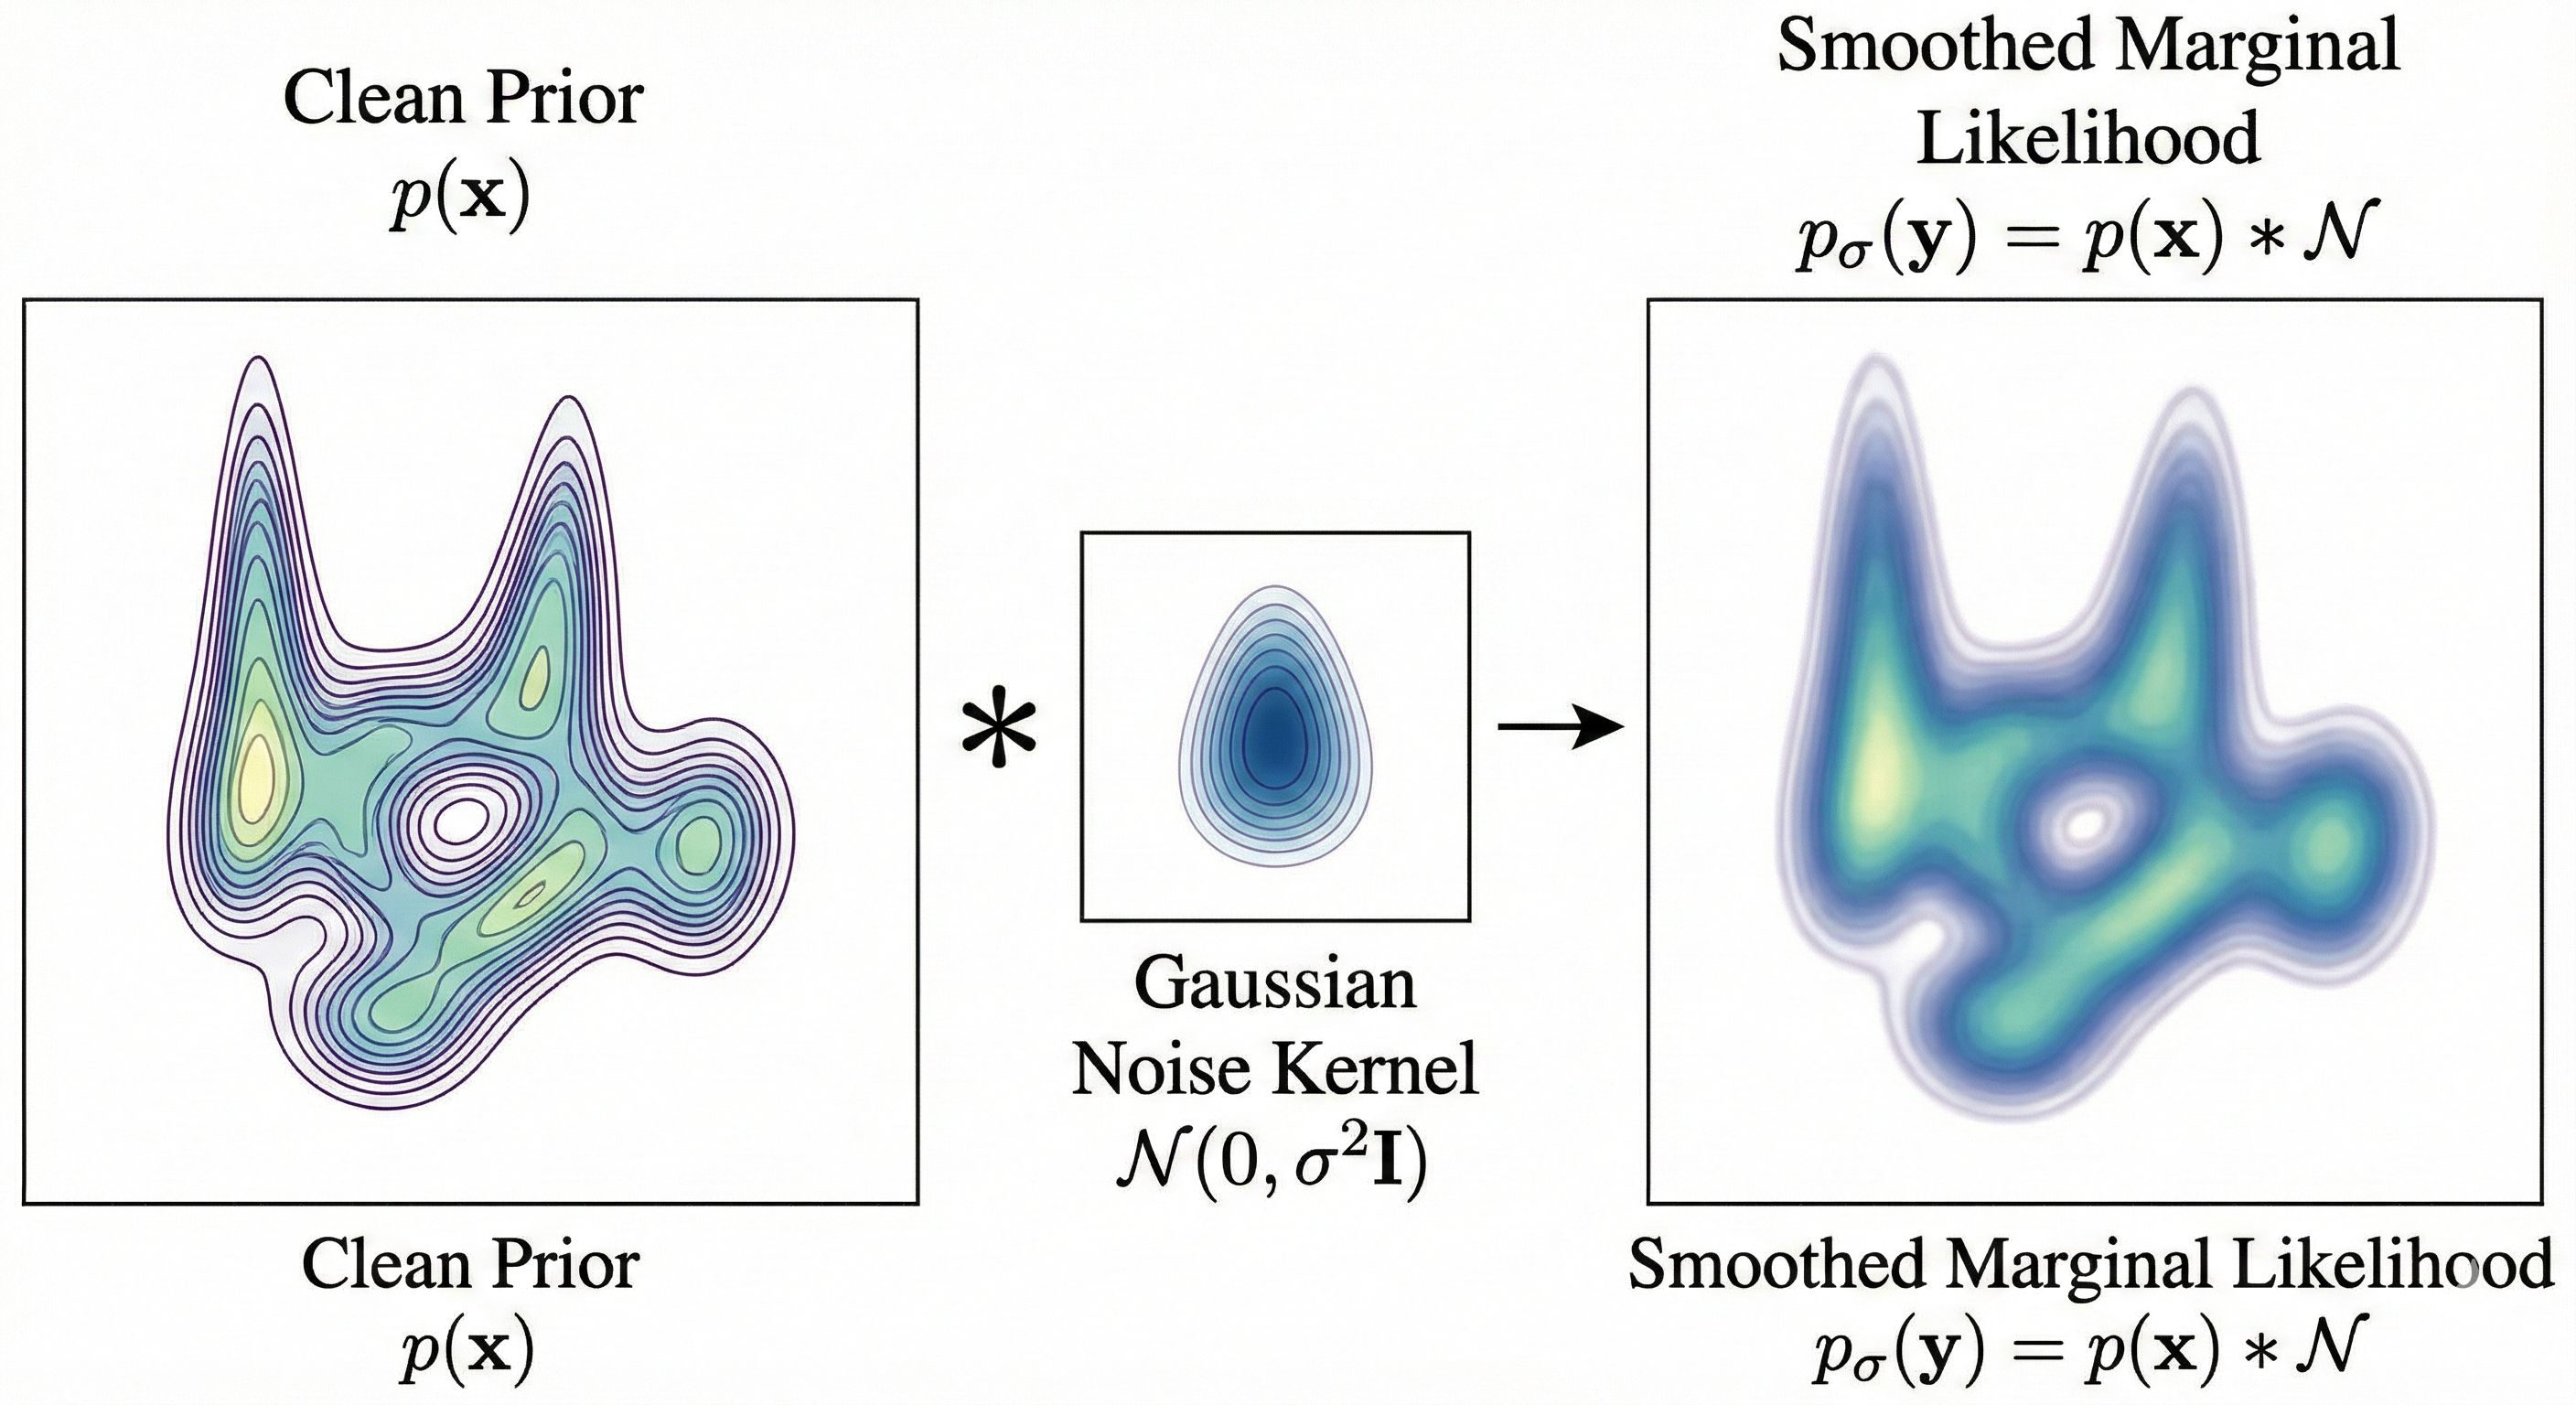
\includegraphics[width=0.5\textwidth]{pnp/smoothed-marginal-likelihood.png}
        \caption{The marginal $p_\sigma(y)$ is a smoothed version of the true prior $p(x)$.}
    \end{figure}
\end{frame}

\begin{frame}{The Problem with the MMSE Estimator}
    To find the MMSE estimator, we must compute the expected value of the posterior:\vspace{1em}
    
    $$ D_\sigma^*(y) = \mathbb{E}[x | y] = \int x \frac{p(y | x) p(x)}{p(y)} \, dx $$
    
    \vspace{1em}
    \textbf{The Fundamental Challenge:} 
    The true prior distribution $p(x)$ for natural images is an unimaginably complex, high-dimensional manifold. We cannot write down a formula for it, making this integral strictly impossible to solve analytically.
\end{frame}

\begin{frame}{Tweedie's Formula: The Derivation (1/2)}
    A profound result from statistics, \textbf{Tweedie's Formula}, proves we can bypass $p(x)$ entirely! 
    
    If we assume additive white Gau\ss ian noise $n \sim \mathcal{N}(0, \sigma^2 I)$, the likelihood reads
    $$ p(y | x) \propto \exp\left( - \frac{\|y - x\|_2^2}{2\sigma^2} \right) \, . $$
    
    Taking the gradient with respect to the observation $y$ yields
    $$ \nabla_y p(y | x) = -\frac{y - x}{\sigma^2} p(y | x) \, . $$
\end{frame}

\begin{frame}{Tweedie's Formula: The Derivation (2/2)}
    Now let us consider the marginal distribution of the noisy data, $p_\sigma(y) = \int p(y | x) p(x) \, dx$. If we take the gradient with respect to $y$ and substitute the likelihood gradient we observe
    \begin{align*}
        \nabla_y p_\sigma(y) &= \int \left( -\frac{y - x}{\sigma^2} \right) p(y | x) p(x) \, dx \, , \\
        \onslide<2->{&= -\frac{1}{\sigma^2} \int (y - x) p(x | y) p_\sigma(y) \, dx \quad \text{(Using Bayes' rule)}} \, , \\
        \onslide<3->{&= -\frac{p_\sigma(y)}{\sigma^2} \left( y \underbrace{\int p(x | y) \, dx}_{=1} - \underbrace{\int x \, p(x | y) \, dx}_{=\mathbb{E}[x | y]} \right)} \, .
    \end{align*}
    
    \onslide<4->{Dividing by $p_\sigma(y)$ and recognising $\frac{\nabla p}{p} = \nabla \log p$, we get Tweedie's Formula.}
\end{frame}

\begin{frame}{Tweedie's Formula: The Result}
    \begin{theoremblock}{Tweedie's Formula}
        $$ \mathbb{E}[x | y] = y + \sigma^2 \nabla_y \log p_\sigma(y) $$
    \end{theoremblock}
    
    \vspace{1em}
    \textbf{Why is this remarkable?} 
    It states that the optimal MMSE denoiser $D_\sigma^*(y) = \mathbb{E}[x | y]$ depends \emph{only} on the gradient of the log-marginal distribution of the \textbf{noisy} data. 
    
    We do not need to know the complex, difficult (or even impossible) to model clean prior $p(x)$!
\end{frame}

\section{Resolving the RED Mystery}

\begin{frame}{Score-Matching by Denoising (SMD)}
    Rearranging Tweedie's formula, we can express the \textbf{score function} (the vector field pointing towards higher probability density) directly in terms of the denoiser's residual:
    
    $$ \nabla_y \log p_\sigma(y) = \frac{D_\sigma^*(y) - y}{\sigma^2} $$
    
    This insight resolves the theoretical crisis of RED discussed in Lecture 2.
    
    Reehorst and Schniter (2018) \cite{reehorst2018regularization} showed that while $u - D(u)$ is not the gradient of a regulariser $\rho(u)$, it \textbf{is} proportional to the score, i.e.,
    
    $$ u - D(u) = -\sigma^2 \nabla_u \log p_\sigma(u) \, . $$
    
    \textbf{Conclusion:} RED and PnP are performing \textbf{Gradient Ascent on the Log-Likelihood} of the smoothed data distribution. They are instances of \emph{Score-Matching by Denoising} \cite{romano2017little, reehorst2018regularization}.
\end{frame}

\section{From PnP to Diffusion Models}

\begin{frame}{The Need for Sampling}
    Deterministic iterative algorithms (PnP, RED) climb the probability landscape to reach a single peak or point of consensus.\vspace{1em}
    
    But inverse problems are often highly ambiguous (e.g., missing pixels, severe blur). There might be dozens of perfectly valid images that match the observation.\vspace{1em}
    
    Instead of finding a single best guess, we want to \textbf{sample} from the posterior distribution $p(u | f^\delta)$ to generate a diversity of valid solutions.
\end{frame}

\begin{frame}{Langevin Dynamics}
    To sample the posterior, we use \textbf{Langevin Dynamics} \cite{welling2011bayesian}, i.e.
    $$ u_{k+1} = u_k + \frac{\tau}{2} \nabla_u \log p(u_k | f^\delta) + \sqrt{\tau} z_k \, . $$

    \begin{columns}
        \begin{column}{0.5\textwidth}
            \begin{itemize}
                \item \textbf{Drift ($\nabla \log p$):} Deterministic force pulling the image towards high-probability modes.
                \item \textbf{Diffusion ($\sqrt{\tau} z_k$):} Stochastic force enabling exploration of the mode's volume.
            \end{itemize}
        \end{column}
        \begin{column}{0.5\textwidth}
            \centering
            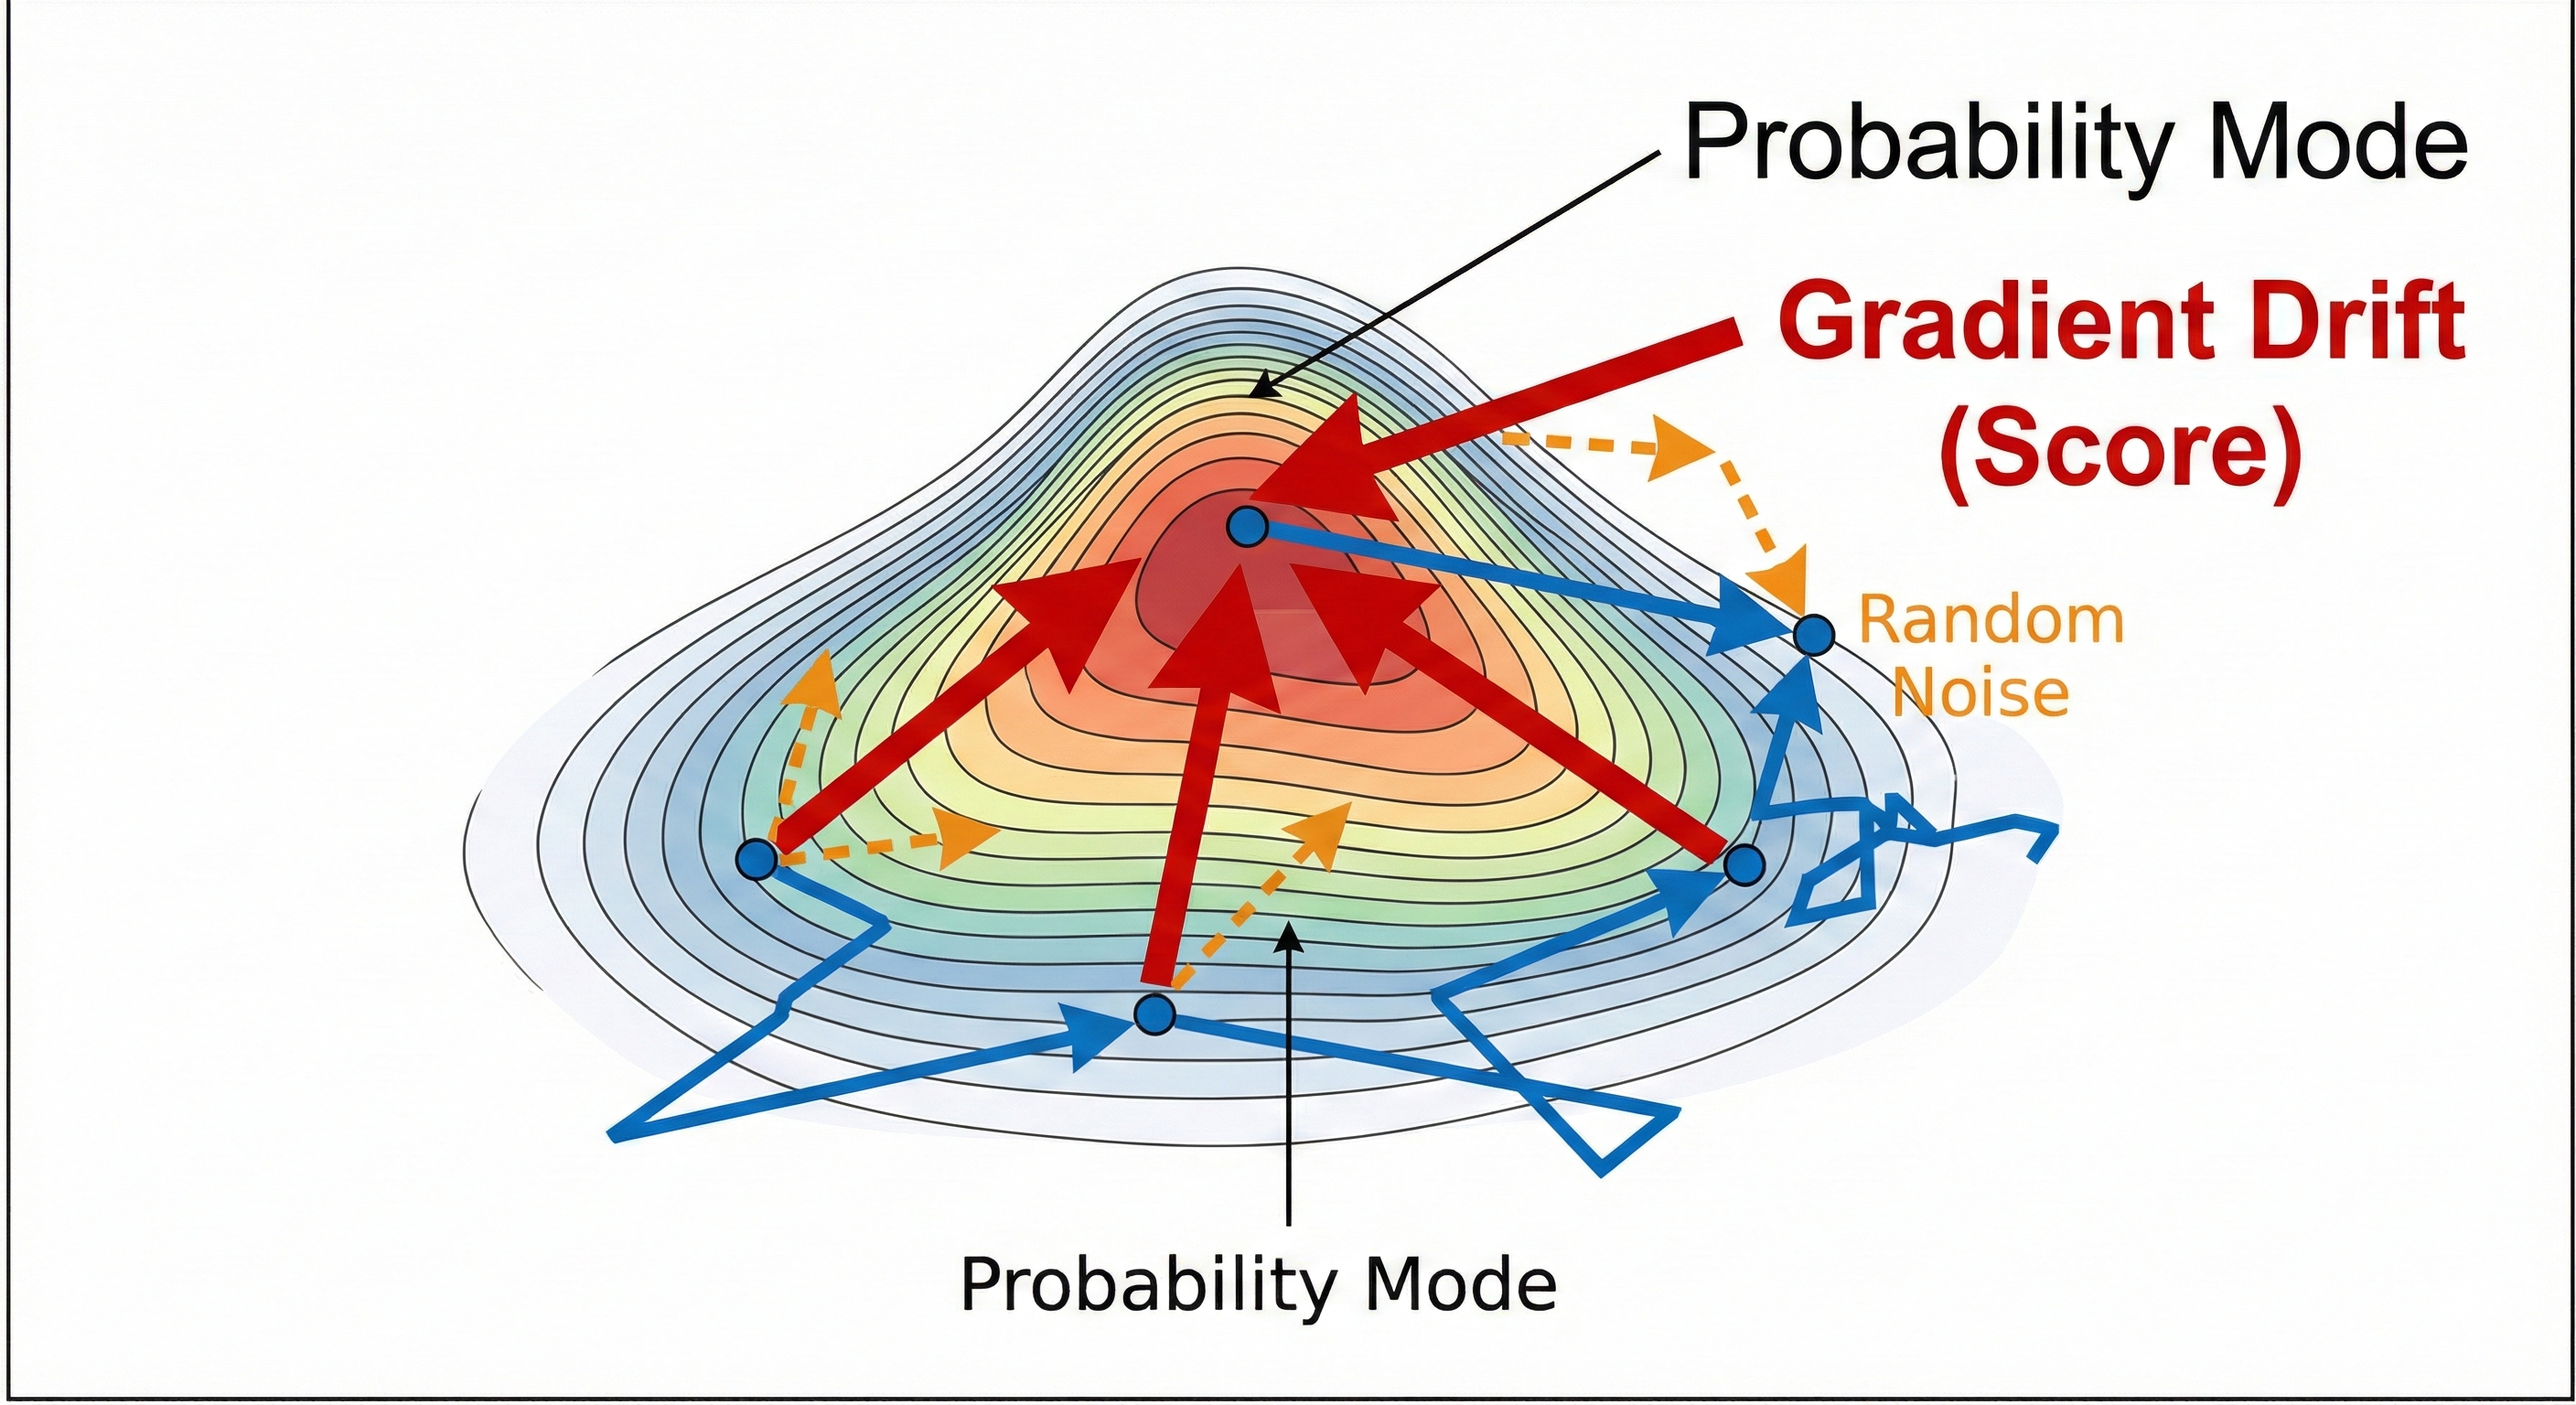
\includegraphics[width=\textwidth]{pnp/langevin-gradient-drift.png}
        \end{column}
    \end{columns}
\end{frame}

\begin{frame}{Decomposing the Posterior Score}
    To use Langevin dynamics, we need the score of the posterior, $\nabla_u \log p(u | f^\delta)$.\vspace{0.1em}
    Using Bayes' rule and taking logarithms we observe
    $$ \log p(u | f^\delta) = \log p(f^\delta | u) + \log p(u) - \log p(f^\delta) \, . $$
    Taking the gradient with respect to $u$ (note that $p(f^\delta)$ vanishes) yields
    $$ \nabla_u \log p(u | f^\delta) = \underbrace{\nabla_u \log p(f^\delta | u)}_{\text{Likelihood Score}} + \underbrace{\nabla_u \log p(u)}_{\text{Prior Score}} \, . $$
    We can substitute our two score components:
    \begin{enumerate}
        \item \textbf{Likelihood Score:} Pushes towards physical measurements. For Gau\ss ian noise, this is $K^\ast (f^\delta - Ku)$.
        \item \textbf{Prior Score:} Pushes towards natural images. By Tweedie's formula, we replace this by $\frac{1}{\sigma^2}(D_\sigma(u) - u)$.
    \end{enumerate}
\end{frame}

\begin{frame}{The PnP-Langevin Update}
    Substituting these into the Langevin update gives us
    
    $$ u_{k+1} = u_k - \frac{\tau}{2} \nabla_u F(Ku_k, f^\delta) + \frac{\tau}{2\sigma^2} \Big( D_\sigma(u_k) - u_k \Big) + \sqrt{\tau} z_k \, . $$
    
    \pause
    \begin{theoremblock}{A Remarkable Connection}
        If we remove the random noise $\sqrt{\tau} z_k$, this is mathematically identical to the gradient descent update for RED!˜vspace{1em} 
        
        By injecting controlled noise into PnP/RED, we transition from classical deterministic solvers to stochastic samplers.
    \end{theoremblock}
\end{frame}

\section{Diffusion Posterior Sampling}

\begin{frame}{The Multi-Modal Trap}
    Running Langevin dynamics at a \emph{fixed} noise level $\sigma$ is practically challenging. True posterior of natural images consists of sharp peaks separated by vast regions of near-zero probability.
    
    \begin{itemize}
        \item \textbf{High $\sigma$:} Easy to move, but distribution is too blurry.
        \item \textbf{Low $\sigma$:} Distribution is sharp, but modes are isolated; the sampler gets trapped.
    \end{itemize}
    
    \begin{figure}
        \centering
        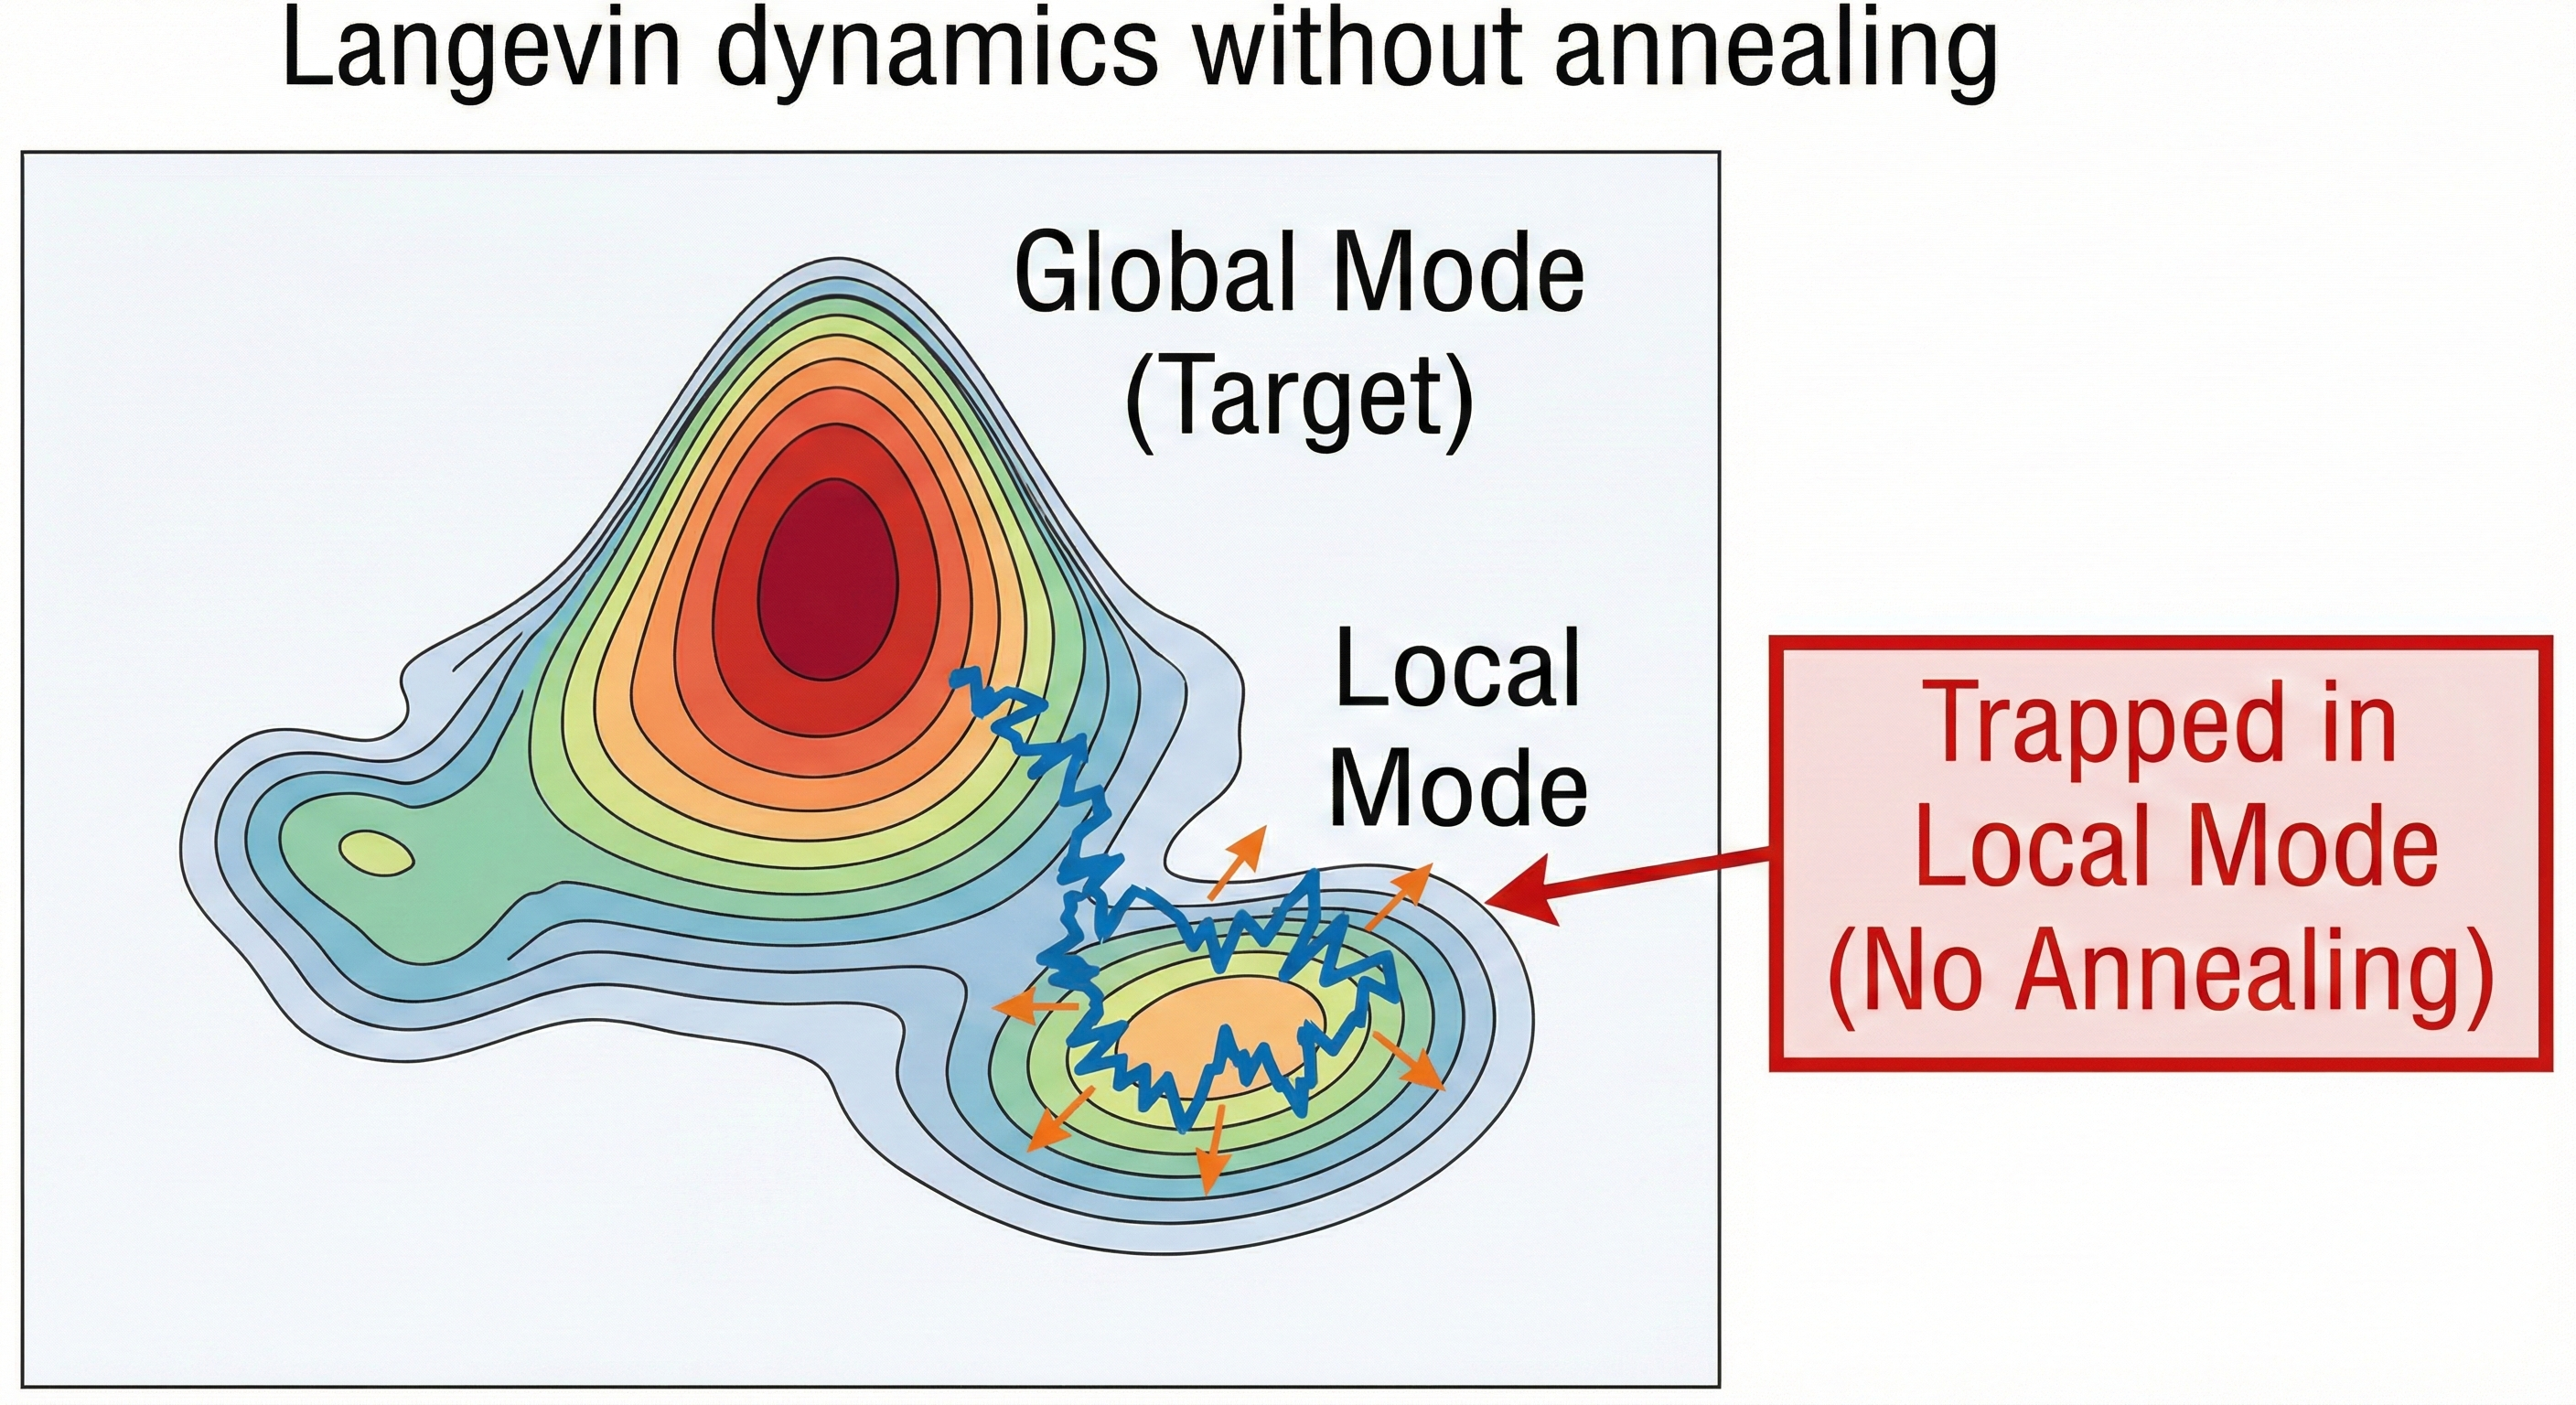
\includegraphics[width=0.55\textwidth]{pnp/langevin-annealing.png}
        \caption{Annealing the noise level allows us to bridge isolated modes.}
    \end{figure}
\end{frame}

\begin{frame}{Annealed Langevin Dynamics (Diffusion)}
    \textbf{Solution:} Define a noise schedule $\sigma_T > \dots > \sigma_0 \approx 0$. We train a time-dependent denoiser $D_{\sigma_t}(u)$ and run the solver using an algorithm known as \textbf{Diffusion Posterior Sampling (DPS)} \cite{chung2023diffusion}, i.e.,
    
    \begin{columns}
        \begin{column}{0.5\textwidth}
            \begin{align*}
                u_{t-1} {} = {} &u_t - \gamma_t \nabla F(K u_t)\\
                &+ \frac{\gamma_t}{\sigma_t^2} (D_{\sigma_t}(u_t) - u_t) + \xi_t z_t
            \end{align*}
        \end{column}
        \begin{column}{0.5\textwidth}
           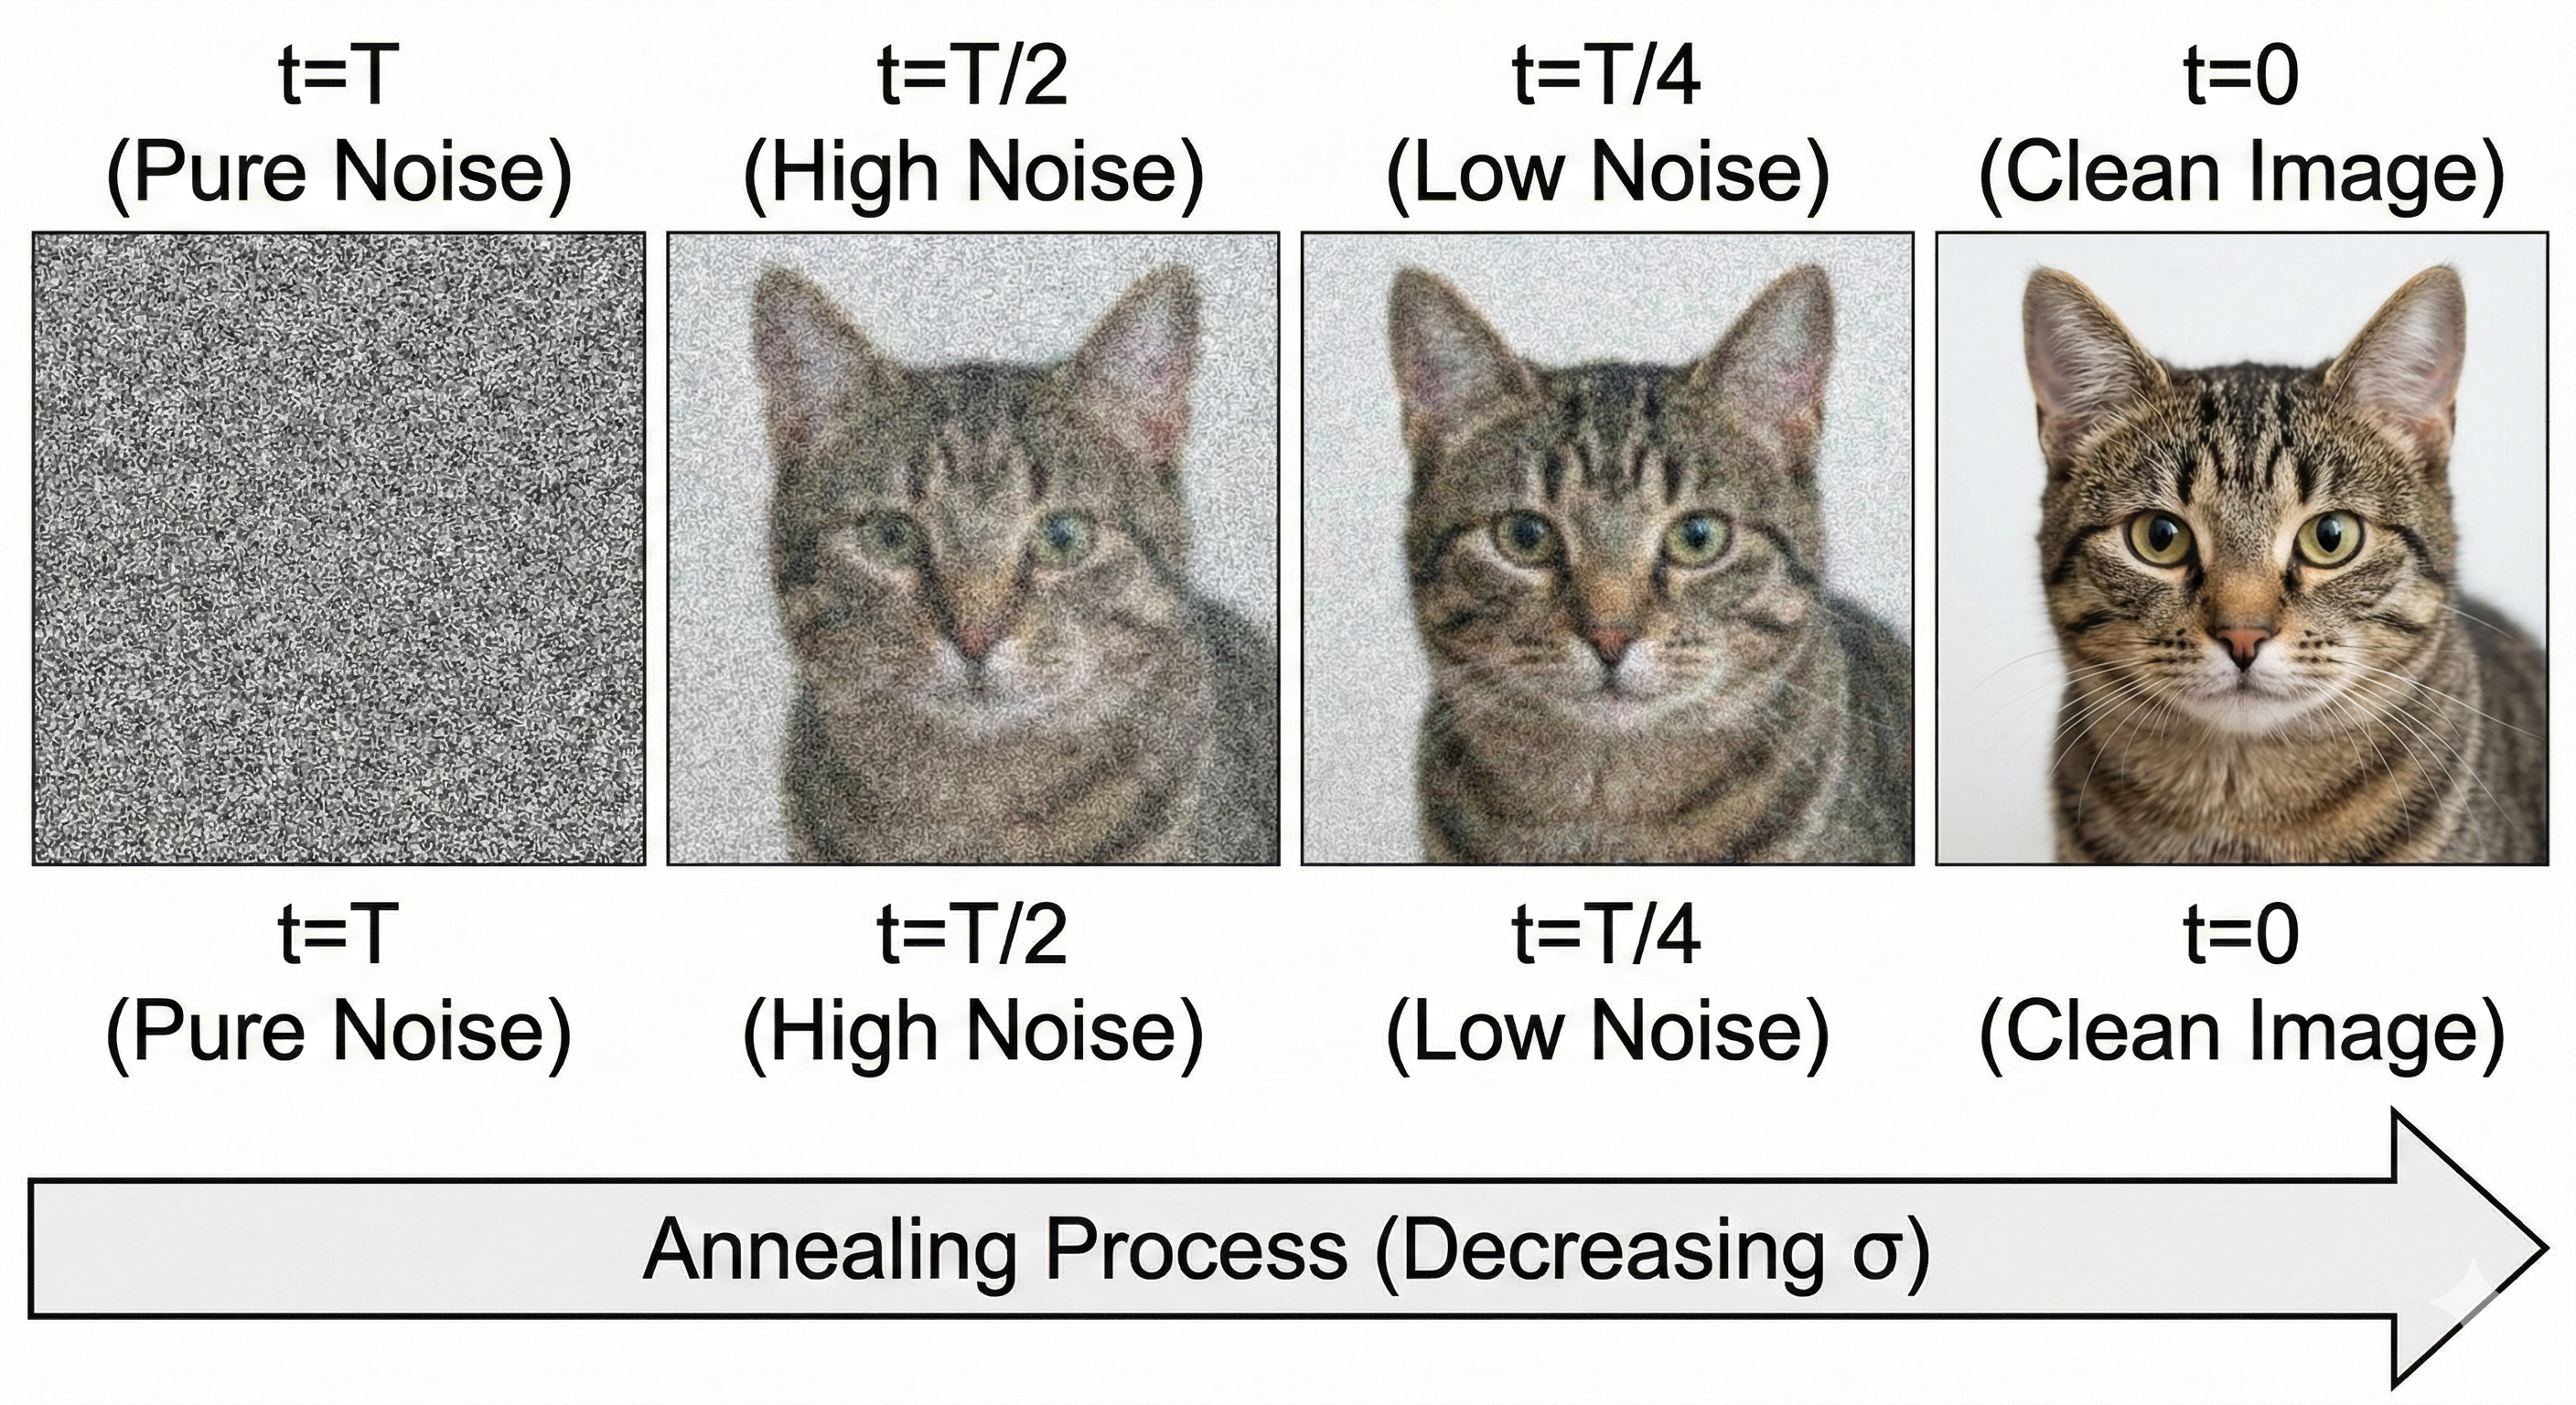
\includegraphics[width=\textwidth]{pnp/noise-schedule.png}
        \end{column}
    \end{columns}
\end{frame}

\section{Summary}

\begin{frame}{Summary of this Week}
    We have completed our journey from classical inverse problems to modern generative AI:
    
    \begin{enumerate}
        \item \textbf{PnP / RED:} Replacing proximal operators with denoisers is not just a trick; it implicitly performs gradient ascent on the data distribution via \textbf{Score Matching} (Tweedie's Formula).
        \item \textbf{Consensus vs Probability:} While early PnP algorithms sought a single deterministic consensus equilibrium, shifting to the probabilistic perspective allows us to understand the uncertainty of the problem.
        \item \textbf{DPS / Diffusion:} By rigorously annealing $\sigma_t$ down to zero and keeping stochastic noise $z_t$, we evolve PnP into a method that generates a full distribution of highly detailed, diverse posterior samples.
    \end{enumerate}
\end{frame}
\begin{frame}[allowframebreaks]{References}
    \bibliographystyle{abbrv}
    \bibliography{../../Lecture_Notes/references}
\end{frame}\end{document}